\section{Results}
\label{sec:results}

\subsection{H1: heads form one population}
\label{sec:h1}

{\bf No run in any configuration bifurcates.} None of the 68 runs meets the criterion under any of the five rank definitions, at 20\% of training or at the end (\tabref{tab:h1}, \figref{fig:heads}). The choice of definition moves the whole population without splitting it: numerical rank puts 99\% of \sst heads above $0.6n$ and stable rank puts all of them below $0.1n$. The dip test reaches $p<.05$ in 3 of 68 runs (4.4\%), about the chance rate, and two of these are shuffled-label runs. Other definitions give 2--4 of 68.

Only \bert has heads above $0.6n$ under $\reff$: 4\% at the start and 3\% at the end, mostly in layers 1, 3, and 4. These heads come from pretraining, not from this training run. Head ordering settles fairly early. The Spearman correlation between a head's rank at 20\% and at the end is 0.70--0.98 in most configurations, with \cfg{ag\_L12} the exception at 0.32. Ordering stabilizes along a continuum, not into two groups.

\begin{figure}[t]
    \centering
    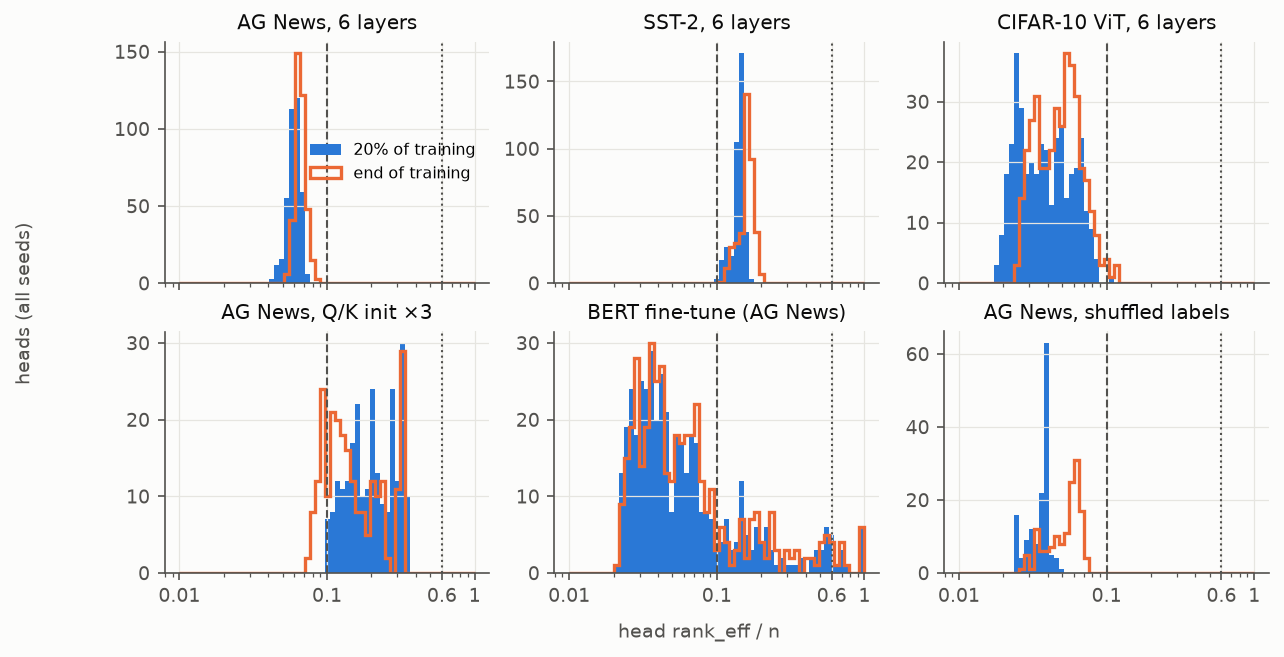
\includegraphics[width=0.95\linewidth]{figures/fig2_heads.png}
    \caption{Distribution of head $\reff/n$ at 20\% of training and at the end, over all seeds. Dashed and dotted lines mark the claimed limits of 0.1 and 0.6. Heads do not form two groups on either side of these limits; the only heads above 0.6 are in pretrained \bert.}
    \label{fig:heads}
\end{figure}

\begin{table}[t]
    \centering
    \small
    \begin{tabular}{@{}lrrrrr@{}}
        \toprule
        \textbf{Configuration} & \textbf{Share $>0.6n$} & \textbf{Share $<0.1n$} & \textbf{Between} & \textbf{Median $\reff/n$} & \textbf{Mean dip $p$} \\
        \midrule
        \cfg{ag\_L6} & 0.000 & 1.000 & 0.000 & 0.060 & .63 \\
        \cfg{sst\_L6} & 0.000 & 0.000 & 1.000 & 0.144 & .83 \\
        \cfg{cifar\_L6} & 0.000 & 0.997 & 0.003 & 0.036 & .74 \\
        \cfg{ag\_L6\_bigqk} & 0.000 & 0.012 & 0.988 & 0.200 & .35 \\
        \cfg{bert\_ag} & 0.030 & 0.778 & 0.192 & 0.047 & .99 \\
        \bottomrule
    \end{tabular}
    \caption{Head populations at 20\% of training, averaged over seeds. H1 needs at least 10\% of heads in both of the first two columns; no configuration comes close.}
    \label{tab:h1}
\end{table}

\begin{figure}[t]
    \centering
    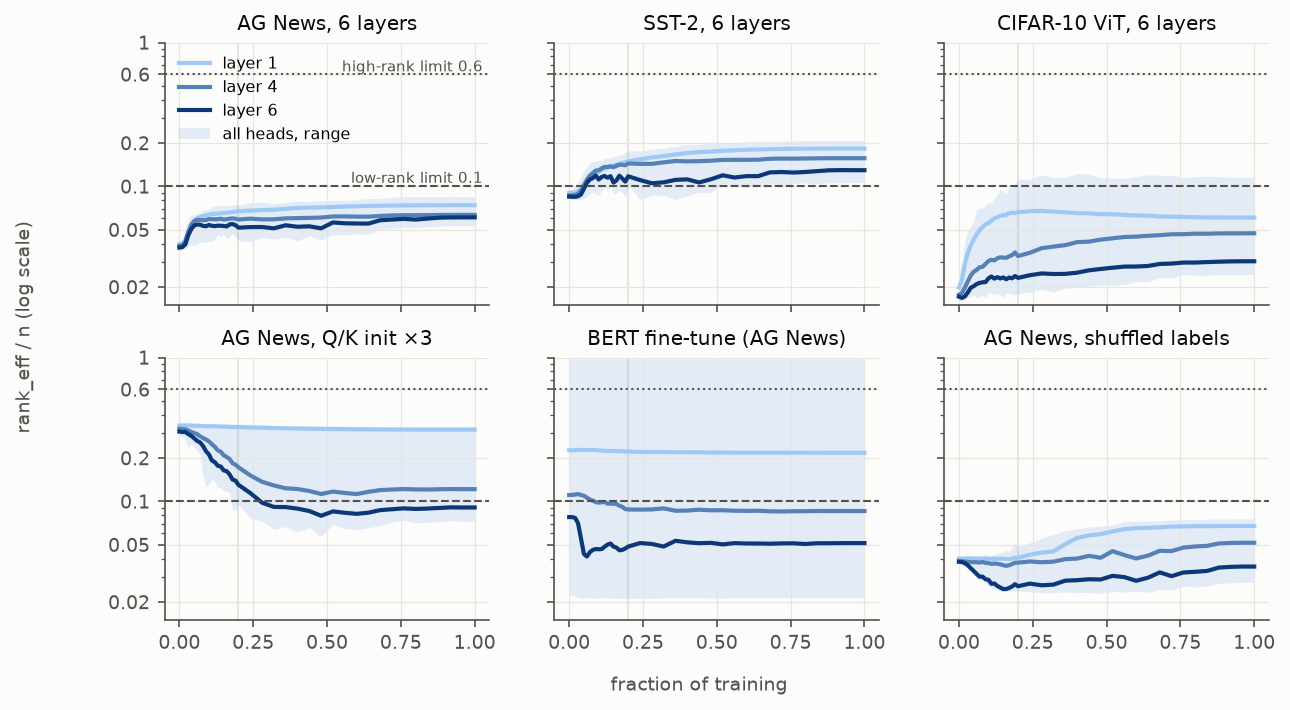
\includegraphics[width=0.95\linewidth]{figures/fig1_rank.png}
    \caption{$\reff/n$ over training on a log scale. Thick lines show first, middle, and last layers (seed means), and the band shows the range over all heads and seeds. Rank rises under default initialization (top row). Later layers lose rank from a peaked start (bottom left) and in pretrained \bert, while first layers keep their initial level. Without label signal (bottom right), the last layer dips and then recovers.}
    \label{fig:rank}
\end{figure}

\subsection{H2: entropy rises under default initialization}
\label{sec:h2}

{\bf The hypothesized pairing of an early monotone fall with a late U-shape occurs in no configuration} (\tabref{tab:h2}, \figref{fig:entropy}). In default arms, no early layer shows a monotone fall, and at most 5\% of late layers show a U-shape. Instead, entropy rises fast. The share of the total rank increase that occurs in the first 10\% of training is 77--86\% on \agnews (all depths and post-LN), 52--60\% on \sst and on \cifar at 3 and 6 layers, and 45\% on \cifar at 12 layers.

A late U-shape does appear in three settings: \cfg{cifar\_L6\_bigqk} (100\% of late layers), \cfg{ag\_L6\_shuffled} (100\%, 3 seeds), and \bert (67\%). It is not tied to large initialization alone, since \cfg{ag\_L6\_bigqk} shows a late fall with no rebound. Rather than a depth law, the U-shape looks like a transient that follows early over-concentration. Early \cifar layers show the opposite of a U: entropy peaks near 40\% of training and then declines slightly.

\begin{table}[t]
    \centering
    \small
    \begin{tabular}{@{}lcccccc@{}}
        \toprule
         & \multicolumn{2}{c}{$S/\log n$, start $\to$ end} & \multicolumn{2}{c}{Early layers} & Late layers \\
        \cmidrule(lr){2-3} \cmidrule(lr){4-5}
        \textbf{Configuration} & \textbf{Early layers} & \textbf{Late layers} & \textbf{Mono.\ fall} & \textbf{Mono.\ rise} & \textbf{U-shape} \\
        \midrule
        \cfg{ag\_L6} & .145 $\to$ .296 & .134 $\to$ .263 & 0\% & 94\% & 0\% \\
        \cfg{sst\_L6} & .159 $\to$ .394 & .143 $\to$ .316 & 0\% & 100\% & 0\% \\
        \cfg{cifar\_L6} & .053 $\to$ .331 & .027 $\to$ .172 & 0\% & 50\% & 0\% \\
        \cfg{ag\_L12} & .142 $\to$ .274 & .118 $\to$ .256 & 0\% & 35\% & 5\% \\
        \cfg{ag\_L6\_bigqk} & .708 $\to$ .636 & .686 $\to$ .353 & 50\% & 0\% & 0\% \\
        \cfg{cifar\_L6\_bigqk} & .367 $\to$ .419 & .322 $\to$ .213 & 0\% & 10\% & 100\% \\
        \cfg{ag\_L6\_shuffled} & .146 $\to$ .273 & .136 $\to$ .136 & 0\% & 50\% & 100\% \\
        \cfg{bert\_ag} & .428 $\to$ .428 & .184 $\to$ .204 & 0\% & 17\% & 67\% \\
        \bottomrule
    \end{tabular}
    \caption{Entropy shapes. Percentages are shares of (seed, layer) cells in the given band of layers. H2 needs a monotone fall early and a U-shape late in the same configuration.}
    \label{tab:h2}
\end{table}

\begin{figure}[t]
    \centering
    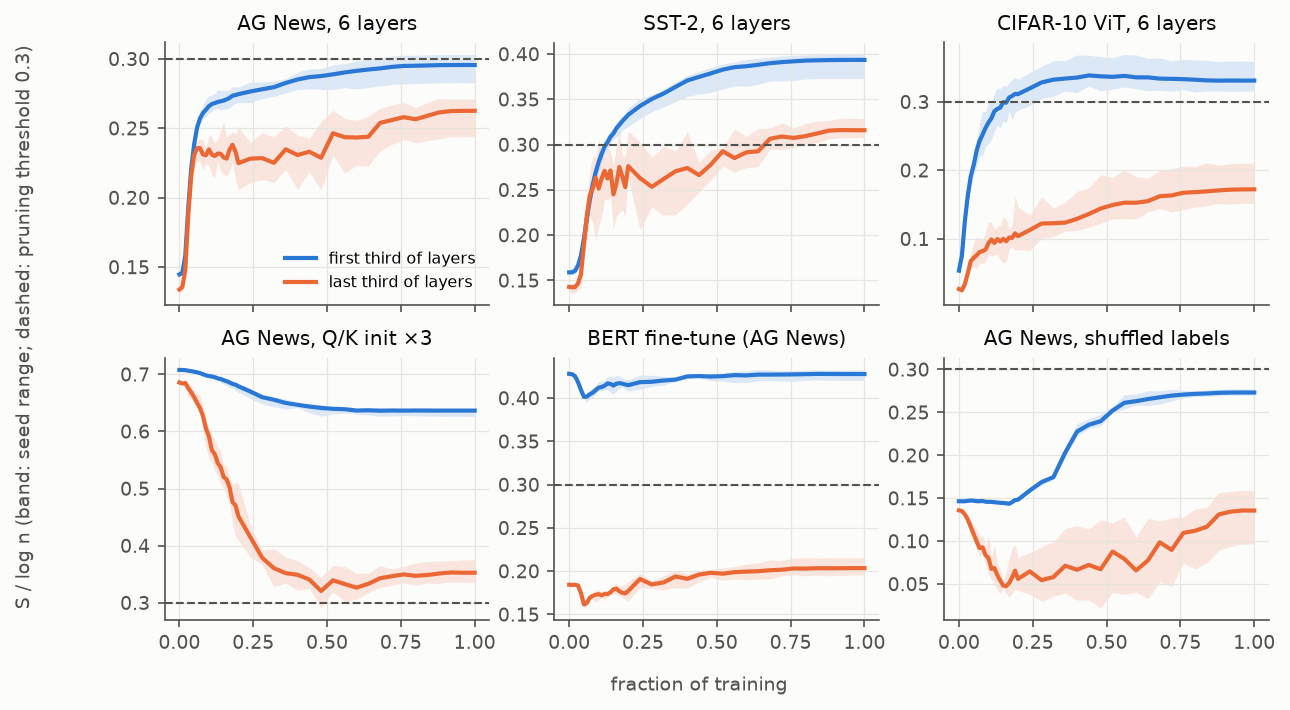
\includegraphics[width=0.95\linewidth]{figures/fig3_entropy.png}
    \caption{$S/\log n$ for the first and last thirds of layers; bands show the seed range and the dashed line marks the 0.3 pruning threshold. Default runs (top row) rise steeply and end near the threshold, which explains why it splits them so poorly (\secref{sec:h3}).}
    \label{fig:entropy}
\end{figure}

\subsection{H3: the threshold is not a safe pruning rule}
\label{sec:h3}

{\bf The rule passes in only 1 of 11 configurations with label signal} (\tabref{tab:h3}). Across \agnews and \cifar default arms it removes 63--96\% of heads at a cost of 19--45\pp. The reason is simple: attention is near-uniform, so most heads lie below $0.3\log n$, and the threshold selects most of the model instead of a redundant minority. \cfg{ag\_L6\_bigqk} has a small loss but prunes only 3.8\% of heads, which fails our non-vacuity rule.

\begin{table}[t]
    \centering
    \small
    \resizebox{\textwidth}{!}{%
    \begin{tabular}{@{}lrrrrrr@{}}
        \toprule
        \textbf{Configuration} & \textbf{Pruned} & \textbf{Low-$S$ loss [95\% CI]} & \textbf{Random} & \textbf{High-$S$} & \textbf{Oracle} & \textbf{Holm $p$ ($<2$\pp)} \\
        \midrule
        \cfg{sst\_L6} & 13.8\% & {\bf 0.12} [$-$0.43, 0.75] & 0.47 & 1.03 & 0.55 & .004 \\
        \cfg{ag\_L6\_bigqk} (vacuous) & 3.8\% & {\bf 0.12} [0.01, 0.27] & 0.24 & 0.22 & 0.26 & $<$.001 \\
        \cfg{ag\_L3} & 95.8\% & 45.3 [42.4, 48.2] & 42.1 & {\bf 39.2} & 43.3 & 1 \\
        \cfg{ag\_L6} & 84.9\% & 19.3 [16.4, 22.0] & {\bf 17.9} & 18.4 & 19.0 & 1 \\
        \cfg{ag\_L12} & 90.2\% & 24.1 [15.9, 31.6] & 25.8 & {\bf 23.7} & 24.2 & 1 \\
        \cfg{ag\_L6\_postln} & 89.2\% & 28.6 [20.4, 39.7] & 26.2 & 30.0 & {\bf 25.1} & 1 \\
        \cfg{cifar\_L3} & 63.3\% & 36.7 [28.2, 44.8] & 40.0 & 47.0 & {\bf 36.6} & 1 \\
        \cfg{cifar\_L6} & 66.9\% & {\bf 32.8} [28.8, 37.1] & 41.3 & 56.5 & 35.6 & 1 \\
        \cfg{cifar\_L12} & 70.0\% & {\bf 27.6} [23.8, 32.2] & 40.3 & 58.5 & 32.5 & 1 \\
        \cfg{cifar\_L6\_bigqk} & 46.7\% & 19.5 [17.5, 21.4] & 22.6 & 46.4 & {\bf 16.2} & 1 \\
        \cfg{bert\_ag} & 64.4\% & 40.9 [15.3, 58.6] & 13.6 & 25.5 & {\bf 7.6} & 1 \\
        \bottomrule
    \end{tabular}}
    \caption{Accuracy loss in percentage points at $\tau=0.3$, with all baselines at the same head count. The lowest loss in each row is in \textbf{bold}. Only \cfg{sst\_L6} passes with a non-vacuous cut. Shuffled-label runs are omitted.}
    \label{tab:h3}
\end{table}

\begin{figure}[t]
    \centering
    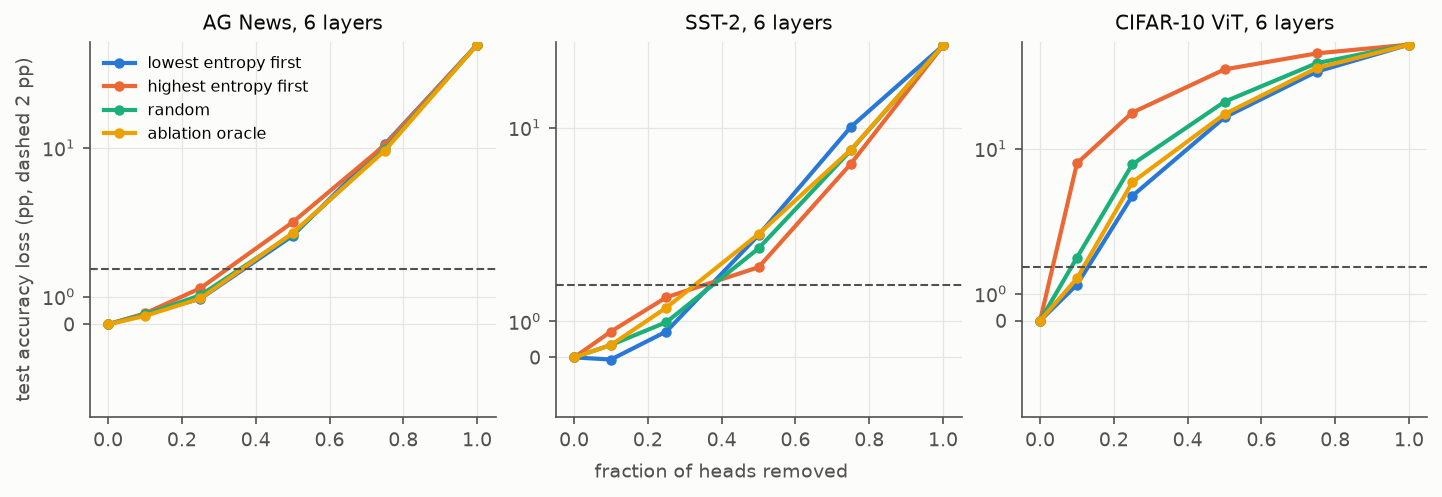
\includegraphics[width=0.95\linewidth]{figures/fig4_prune.png}
    \caption{Accuracy loss against share of heads removed for six-layer models, on a symmetric-log axis; the dashed line marks 2\pp. On \cifar, removing high-entropy heads first is far worse than the other rules, while on \agnews all rules coincide.}
    \label{fig:prune}
\end{figure}

\para{\sst.} The loss meets the criterion, but entropy adds nothing here: the difference from random is $-0.36$\pp (Wilcoxon $p=.25$). With 436 test sentences, one sentence is 0.23\pp, so this comparison is weak. \sst's normalized entropy ends higher than \agnews's (.32--.39 against .26--.30), so few heads fall below the line. Its sequences are also about half as long (mean $n$ of 22 against 46), and we did not test whether length is the cause.

\para{Entropy is a real signal on \cifar but not on text.} At the threshold's head count, removing low-entropy heads first beats random on all three default \cifar depths: by 8.5\pp at $L=6$ (Wilcoxon $p=.008$), 12.7\pp at $L=12$ ($t$-test $p=.005$), and 3.2\pp at $L=3$ ($t$-test $p=.002$). Removing high-entropy heads first costs far more, 56.5\pp against 32.8\pp at $L=6$. The Spearman correlation of $S$ with ablation importance is $+0.23$ to $+0.40$ on \cifar and $-0.14$ to $+0.11$ on default-initialization text. On \agnews, low-$S$ pruning is if anything worse than random, by 1.4\pp at $L=6$ (Wilcoxon $p=.016$). On \bert it is worse by 27\pp, though imprecisely (3 seeds, $t$-test $p=.12$). The ablation oracle does not always win, because single-head importance is a poor guide to joint removal.

\para{Smaller cuts and fine-tuning.} When we cut only 25\% of heads, default \agnews models and \sst lose 0.7--1.7\pp under every selection rule. This echoes \citet{michel2019sixteen}: much head removal is cheap under any method. \cifar at $L=6$ is different, losing 4.6\pp with low-$S$ first and 19.8\pp with high-$S$ first. Fine-tuning recovers much of the loss but not enough: \agnews goes from 19.3 to 10.4\pp and \cifar from 32.8 to 8.5\pp, while \sst stays at 0.12\pp.

\subsection{H4: the bound is false}
\label{sec:h4}

\begin{proposition}[Counterexample]
\label{prop:counter}
Let $X$ be uniform on $M\ge2$ inputs and $Y=f(X)$, so $H(Y|X)=0$. Take any network that computes $f$ and has a head whose attention map $x\mapsto\mA(x)$ is injective on these inputs, with that head's output weight set to zero. Predictions are unaffected, and since $\mA$ is a function of $X$, $I(\mA;X)=H(\mA)=\log M$ for every $n$. The right side of the claim tends to 0.
\end{proposition}

The training-set size cannot rescue the claim: $I(\mA;X)$ is a property of the map, and nothing forces a Bayes-optimal network's attention to discard input information. The direction is also suspect. The data-processing inequality gives $I(\mA;Y)\le I(X;Y)=H(Y)-H(Y|X)$, which falls with $H(Y|X)$, whereas the claim rises with it.

\begin{proposition}[Variance bound]
\label{prop:variance}
For $T=\mA(X)+\epsilon Z$ with $Z$ standard Gaussian and $\bar\mA=\E\,\mA(X)$,
\begin{equation*}
I(T;X)\le\min\Big\{\log M,\ \frac{\E\|\mA(X)-\bar\mA\|_F^2}{2\epsilon^2}\Big\}.
\end{equation*}
\end{proposition}
\begin{proof}
$I(T;X)=\E\,\mathrm{KL}(\gN(\mA(X),\epsilon^2I)\,\|\,P_T)\le\E\,\mathrm{KL}(\gN(\mA(X),\epsilon^2I)\,\|\,\gN(\bar\mA,\epsilon^2I))$, because the true marginal $P_T$ minimizes the expected KL over all reference distributions. The right side equals the variance term. The $\log M$ term follows from $I(T;X)\le H(X)$.
\end{proof}

What bounds the information is attention variability relative to the noise, and $H(Y|X)$ does not appear. $\Ibd$ stayed below this bound in all 19,200 checks (every layer, noise scale, and checkpoint). $\Ikl$ may exceed it, since Jensen's inequality only gives $\Ikl\le2\times$ the bound, and it does so at $\epsilon=2$.

\para{Measurements.} \Tabref{tab:h4} and \figref{fig:mi} show noise-free results. At $H(Y|X)=0$ and 100\% accuracy on \order ($n=32{,}000$), layer-level information is at least 1.04 nats on average, where the claim allows only $C/179$. Seeds vary widely here, from 0.21 to 1.83 nats. The per-head mean is 0.13 nats.

{\bf The excess does not shrink with $n$.} A true $O(1/\sqrt n)$ term needs a bounded $C$. On \agnews the implied $C$ rises from 7 to 180 at the layer level and from 0.9 to 23 at the head level. On \order it rises non-monotonically, from 40 to 186 and from 5 to 24. The \order trend is noisy and its $n=500$ cell did not learn the task, so \agnews carries more of the weight here. The regression also fails at every scale (\tabref{tab:regression}). Where the interval for $b$ includes 1 in the layer-level fits, the intercept is 1.4--5.5 nats, not near zero. On \agnews, $c$ is negative at every scale: information rises with $n$, the opposite of the claimed term.

{\bf Single numbers depend on the level and the noise scale.} At $\epsilon=2$, layer-level $\Ibd$ exceeds $H(Y|X)+1/\sqrt n$ in 93\% of \order runs and 73\% of \agnews runs. For the per-head mean these shares fall to 35\% and 15\%, and at $\epsilon=1$ they are 90\% and 47\%. Large noise can make the claim pass trivially: at $\epsilon=4$, noise-free \order runs at $n=8{,}000$ reach 0.13 nats. Cells below the claimed value are mostly noisy ones, such as \agnews at $\eta=0.4$, $n=500$ (0.32 against 1.11 nats), and these are consistent with the claim only because information is low there, not because it tracks $H(Y|X)$. An untrained network already exceeds the claim at low noise (\agnews at $\epsilon=1$: $\Ibd=0.65$ nats at step 0). For these reasons we rest the refutation on Proposition~\ref{prop:counter} and on the trend in $n$, and not on any one number.

Label noise does raise information, which fits the claim in sign only: at $n=32{,}000$ on \agnews, $\Ibd$ goes from 1.0 to 2.7 nats as $\eta$ goes from 0 to 0.4. Memorization of noisy labels is a likely mechanism, though we did not test it. Saturation is partial. At $n=8{,}000$, \agnews plateaus by 40\% of training and noise-free \order by 20\%, while \order at $\eta=0.2$ keeps rising (0.5 nats at 20\%, 3.8 at 60\%, 4.4 at the end). Plateaus do not sit at $H(Y|X)$.

\begin{figure}[t]
    \centering
    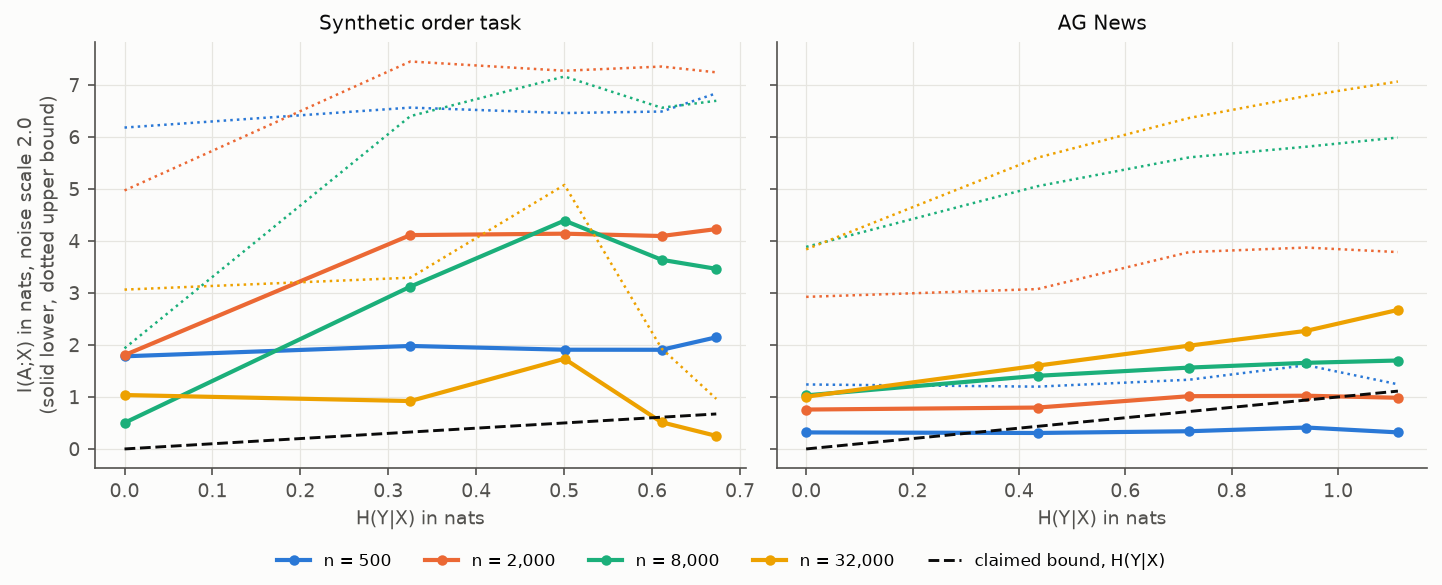
\includegraphics[width=0.95\linewidth]{figures/fig5_mi.png}
    \caption{Estimated layer-level information at $\epsilon=2$, averaged over layers and seeds. Solid lines are the lower bound and dotted lines the upper bound. The dashed black line is the claimed $H(Y|X)$ with the $O(1/\sqrt n)$ term set to zero. Noise-free points (left end) lie above the line at every $n$, and the curves do not approach it as $n$ grows.}
    \label{fig:mi}
\end{figure}

\begin{table}[t]
    \centering
    \small
    \begin{tabular}{@{}lrrrr@{}}
        \toprule
        \textbf{Noise-free runs, $\epsilon=2$} & \textbf{$n=500$} & \textbf{$n=2{,}000$} & \textbf{$n=8{,}000$} & \textbf{$n=32{,}000$} \\
        \midrule
        \order: layer $\Ibd$, nats (test accuracy) & 1.78 (49\%) & 1.80 (99\%) & 0.50 (100\%) & 1.04 (100\%) \\
        \order: implied $C$, layer / head & 40 / 5 & 81 / 10 & 45 / 6 & 186 / 24 \\
        \midrule
        \agnews: layer $\Ibd$, nats (test accuracy) & 0.32 (63\%) & 0.76 (76\%) & 1.03 (83\%) & 1.01 (87\%) \\
        \agnews: implied $C$, layer / head & 7 / 0.9 & 34 / 4 & 92 / 12 & 180 / 23 \\
        \bottomrule
    \end{tabular}
    \caption{Noise-free information. Implied $C$ is the excess of $\Ibd$ over $H(Y|X)$ times $\sqrt n$, which a true $O(1/\sqrt n)$ term would keep bounded. ``Layer'' treats all 8 heads jointly; ``head'' is the mean over heads.}
    \label{tab:h4}
\end{table}

\subsection{H5: depth shapes the size of the fall more than its speed}
\label{sec:h5}

\begin{table}[t]
    \centering
    \small
    \resizebox{\textwidth}{!}{%
    \begin{tabular}{@{}lccccl@{}}
        \toprule
        \textbf{Configuration} & \textbf{$t_{\min}$ layer 1} & \textbf{$t_{\min}$ last} & \textbf{Ratio [95\% CI]} & \textbf{Rank drop, first $\to$ last} & \textbf{Reading} \\
        \midrule
        \cfg{ag\_L3}, \cfg{ag\_L6}, \cfg{cifar\_L3} & 0 & 0 & undefined & 0 (rank rises) & Minimum at initialization \\
        \cfg{ag\_L12}, \cfg{cifar\_L6}, \cfg{cifar\_L12}, \cfg{sst\_L6} & $\le$.001 & .010--.124 & $\approx$0 & $\approx$0 & Same \\
        \cfg{ag\_L6\_bigqk} & .69 & .38 & {\bf 1.81} [1.63, 2.00] & 7\% $\to$ 75\% & Real collapse, below $3\times$ \\
        \cfg{cifar\_L6\_bigqk} & .002 & .14 & 0.01 [0, .04] & 0.4\% $\to$ 60\% & Layer 1 never falls \\
        \cfg{bert\_ag} & .63 & .05 & 11.9 [10.0, 14.4] & 4\% $\to$ 47\% & Layer 1 barely falls; unstable \\
        \bottomrule
    \end{tabular}}
    \caption{Time to minimum rank as a fraction of training. The criterion needs a fall of at least 10\% in both layers. No run in any configuration satisfies this.}
    \label{tab:h5}
\end{table}

{\bf Under default initialization there is no collapse to time} (\tabref{tab:h5}). The minimum sits at or near the start, because rank rises: $\reff/n$ goes from .04 to .07 on \agnews (layer 1), .09 to .18 on \sst, and .02 to .06 on \cifar. Three signal configurations show a real fall in deep layers. \cfg{ag\_L6\_bigqk} gives the only interpretable ratio, 1.81, which is below the claimed range, and even there layer 1 falls only 7\%. In \cfg{cifar\_L6\_bigqk} and \bert, layer 1 hardly falls, so the ratio has little meaning. Without label signal, the last layer of \cfg{ag\_L6\_shuffled} drops 37\% and then recovers, so a transient fall does not need a peaked start.

Post-hoc rise times to peak rank have no consistent sign (\figref{fig:depth}). The mean per-seed ratios of layer 1 to last layer are 7.8, 2.1, and 0.63 on \agnews for $L=3,6,12$, and 0.42, 0.26, and 0.21 on \cifar. The value of 2.1 hides heavy tails: its median is 0.78. \sst gives 3.7 [2.4, 5.0], which overlaps the claimed range, but this measures a different quantity on a post-hoc basis.

{\bf What holds up is the size of the fall.} From a peaked start, the rank drop grows steadily with depth: 7, 36, 56, 66, 70, and 75\% from layer 1 to 6 on \agnews, and 0.4, 14, 30, 42, 53, and 60\% on \cifar. \bert's 4\% to 47\% matches this pattern. In addition, the first layer has higher rank than the last at 95--100\% of checkpoints in every configuration, though not always in strict order across intermediate layers. This agrees with \citet{wang2020linformer}, who report more skewed spectra in higher layers.

\begin{figure}[t]
    \centering
    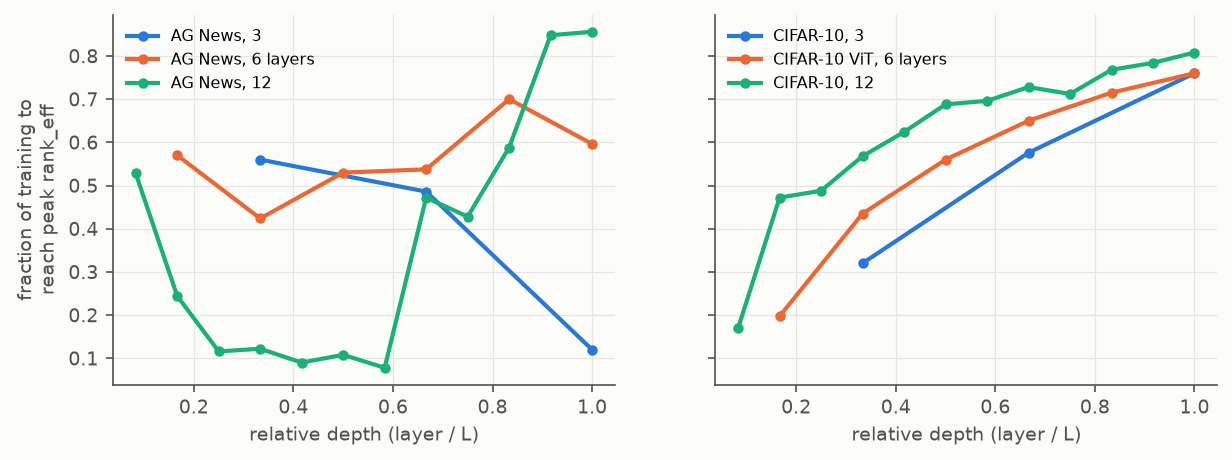
\includegraphics[width=0.8\linewidth]{figures/fig6_depth.png}
    \caption{Fraction of training needed for $\reff$ to reach its peak, by relative depth and network size, under default initialization. \cifar peaks later in deeper layers, while \agnews shows no consistent order. The direction of the depth effect depends on the task.}
    \label{fig:depth}
\end{figure}
